\section{StudentMember-klassen}
\begin{minipage}[t]{1\linewidth}
%Set imagepath and scaling, imagepath set to start in images/UmlMini folder, just write filename and extension
%FBox added for outline on items
\begin{wrapfigure}{l}{0.5\textwidth}
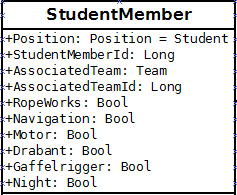
\includegraphics[scale=0.3]{StudentMember_UML.png}
\end{wrapfigure}

'StudentMember' klassen arver fra 'SailClubMember' klassen og fungerer som en elev på et skolehold. Denne klasses 'Position' bliver altid sat til at være 'Student'. 'AssociatedTeam' henviser til det skolehold, den pågældende elev hører til. De seks bool-værdier: 'RopeWorks', 'Navigation', 'Motor', 'Drabant', 'Gaffelrigger' og 'Night' repræsentere et læringsområde og de bliver sat til 'true' når området er lært.

\end{minipage}


\section{Team-klassen}
\begin{minipage}[t]{1\linewidth}
%Set imagepath and scaling, imagepath set to start in images/UmlMini folder, just write filename and extension
%FBox added for outline on items
\begin{wrapfigure}{l}{0.5\textwidth}
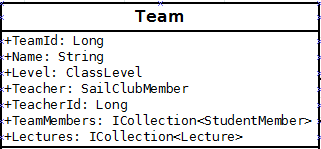
\includegraphics[scale=0.7]{Team_UML.png}
\end{wrapfigure}

'Team' klassen fungerer som et skolehold. 'TeamId' bruges til at identificere de enkelte hold fra hinanden. 'Teacher' er den lærer der er tilknyttet holdet. 'Name' er navnet på holdet. 'Level' fortæller om holdet er et første eller andet års hold. Klassen har en ``collection'' ('TeamMembers') som der bliver sat 'StudentMembers' ind på, hvilket repræsenterer de elever der er på skoleholdet. ``Collectionen'' 'Lectures' indeholder de lektioner som klassen har haft og skal have. 

\end{minipage}
\fxnote{Er ikke sikker på dette, det skal omskrives ud fra hvad der bliver skrevet om 'Lecture'-klassen}

